\documentclass[zihao = -4, linespread = 1.5]{article}

\usepackage[heading = true]{ctex}
\usepackage[bottom]{footmisc}
\usepackage[table]{xcolor}
\usepackage{bm}
\usepackage{tikz}
\usepackage{xeCJK}
\usepackage{float}
\usepackage{natbib}
\usepackage{pifont}
\usepackage{datetime}
\usepackage{geometry}
\usepackage{booktabs}
\usepackage{pdfpages}
\usepackage{fancyhdr}
\usepackage{hyperref}
\usepackage{graphicx}
\usepackage{multirow}
\usepackage{multicol}
\usepackage{makecell}
\usepackage{enumitem}
\usepackage{setspace}
\usepackage{pgfplots}
\usepackage{listings}
\usepackage{threeparttable}
\usepackage{amsmath, amssymb, amsfonts, mathrsfs}

\newCJKfontfamily\JiangChengXieSongTi[Path = ./fonts/]{Italic-SimSun.ttf}
\xeCJKDeclareCharClass{CJK}{"2460 -> "24FF}
\newcommand{\itsongti}[1]{{\JiangChengXieSongTi#1}}

\pgfplotsset{compat = 1.18}
\usepgfplotslibrary{groupplots}
\usetikzlibrary{decorations.pathreplacing, arrows.meta, positioning, calc}

\definecolor{cadetblue}{HTML}{5F9EA0}
\definecolor{deepred}{RGB}{178, 34, 34}
\definecolor{deepblue}{RGB}{40, 115, 180}
\definecolor{darksalmon}{rgb}{0.91, 0.59, 0.48}
\definecolor{forestgreen}{rgb}{0.13, 0.55, 0.13}

\definecolor{grad1}{HTML}{F2E9E4}
\definecolor{grad2}{HTML}{EAE0D5}
\definecolor{grad3}{HTML}{D5DBCB}
\definecolor{grad4}{HTML}{C6D5C5}
\definecolor{grad5}{HTML}{A3B5A5}
\definecolor{grad6}{HTML}{82B0AA}
\definecolor{grad7}{HTML}{66969A}
\definecolor{grad8}{HTML}{4A8B93}
\definecolor{grad9}{HTML}{2A6D79}
\definecolor{grad10}{HTML}{00505F}

\definecolor{mred1}{HTML}{F2EBE9}
\definecolor{mred2}{HTML}{E0C0B8}
\definecolor{mred3}{HTML}{C08E83}
\definecolor{mred4}{HTML}{9E695D}
\definecolor{mred5}{HTML}{6B3E35}

\definecolor{MorandiLightCyan}{RGB}{209, 238, 238}
\definecolor{MorandiBlue}{RGB}{70, 110, 255}
\definecolor{MorandiGrey}{RGB}{80, 100, 100}
\definecolor{MorandiPurple}{RGB}{140, 110, 180}
\definecolor{MorandiCyan}{RGB}{110, 170, 190}
\definecolor{MorandiRed}{RGB}{220, 130, 130}
\definecolor{MorandiOrange}{RGB}{250, 210, 160}

% \AtBeginDocument{
%     \setlength{\abovedisplayskip}{4pt plus 2pt minus 2pt}
%     \setlength{\belowdisplayskip}{4pt plus 2pt minus 2pt}
%     \setlength{\abovedisplayshortskip}{4pt plus 1pt}
%     \setlength{\belowdisplayshortskip}{4pt plus 1pt}
% }

\geometry{
    a4paper,
    top = 2.54cm,
    bottom = 2.1cm,
    left = 2.5cm,
    right = 2.5cm,
    headheight = -1em
}

% \setitemize[1]{
%     itemsep = 0pt,
%     partopsep = 0pt,
%     parsep = \parskip,
%     topsep = 5pt,
%     leftmargin = 2em,
%     labelsep = 0.25em
% }

% \setenumerate[1]{
%     itemsep = 0pt,
%     partopsep = 0pt,
%     parsep = \parskip,
%     topsep = 5pt,
%     leftmargin = 2em,
%     labelsep = 0.25em
% }

\setlist[1]{
    itemsep = 0pt,
    partopsep = 0pt,
    parsep = \parskip,
    topsep = 0pt,
    leftmargin = 2em,
    labelsep = 0.5em
}

\pagestyle{fancy}
\fancyhf{}
\renewcommand{\headrulewidth}{0pt}
\chead{\raisebox{-3em}{\includegraphics*[scale=0.1]{./figs/logo.png}}}
\renewcommand{\thefootnote}{\textcolor{deepred}{\arabic{footnote}}}
\renewcommand{\footnoterule}{\kern -3pt \hrule width 0.75\textwidth height 0.5pt \kern 3pt}

\newcommand{\upcite}[1]{\textsuperscript{\textsuperscript{\cite{#1}}}}
\bibpunct{(}{)}{;}{a}{\textcolor{deepblue}{,}}{,}

\hypersetup{
    colorlinks = true,
    citecolor = deepblue,
    linkcolor = deepred,
    urlcolor = deepred
}

\newcolumntype{C}[1]{>{\centering\arraybackslash}p{#1}}
\newcolumntype{M}[1]{>{\centering\arraybackslash}m{#1}}

\ctexset{
    section = {
        number = \arabic{section},
        format = \zihao{3}\bfseries\raggedright,
        aftername = \hspace{1em}
    },
    subsection = {
        format = \zihao{-3}\bfseries\raggedright,
        aftername = \hspace{1em}
    },
    subsubsection = {
        format = \zihao{4}\bfseries\raggedright,
        aftername = \hspace{1em}
    }
}

\newcommand{\cube}[1]{
    \begin{tikzpicture}[baseline = 0ex]
        \draw[
            draw = #1,
            fill = #1!20,
            thick,
            rounded corners = 0.5pt
        ] (0,0) rectangle (0.25, 0.25);
    \end{tikzpicture}
}
\newcommand{\barline}[1]{\overline{#1\rule{0pt}{1.5ex}}}
\renewcommand{\d}{\mathrm{d}}



\begin{document}



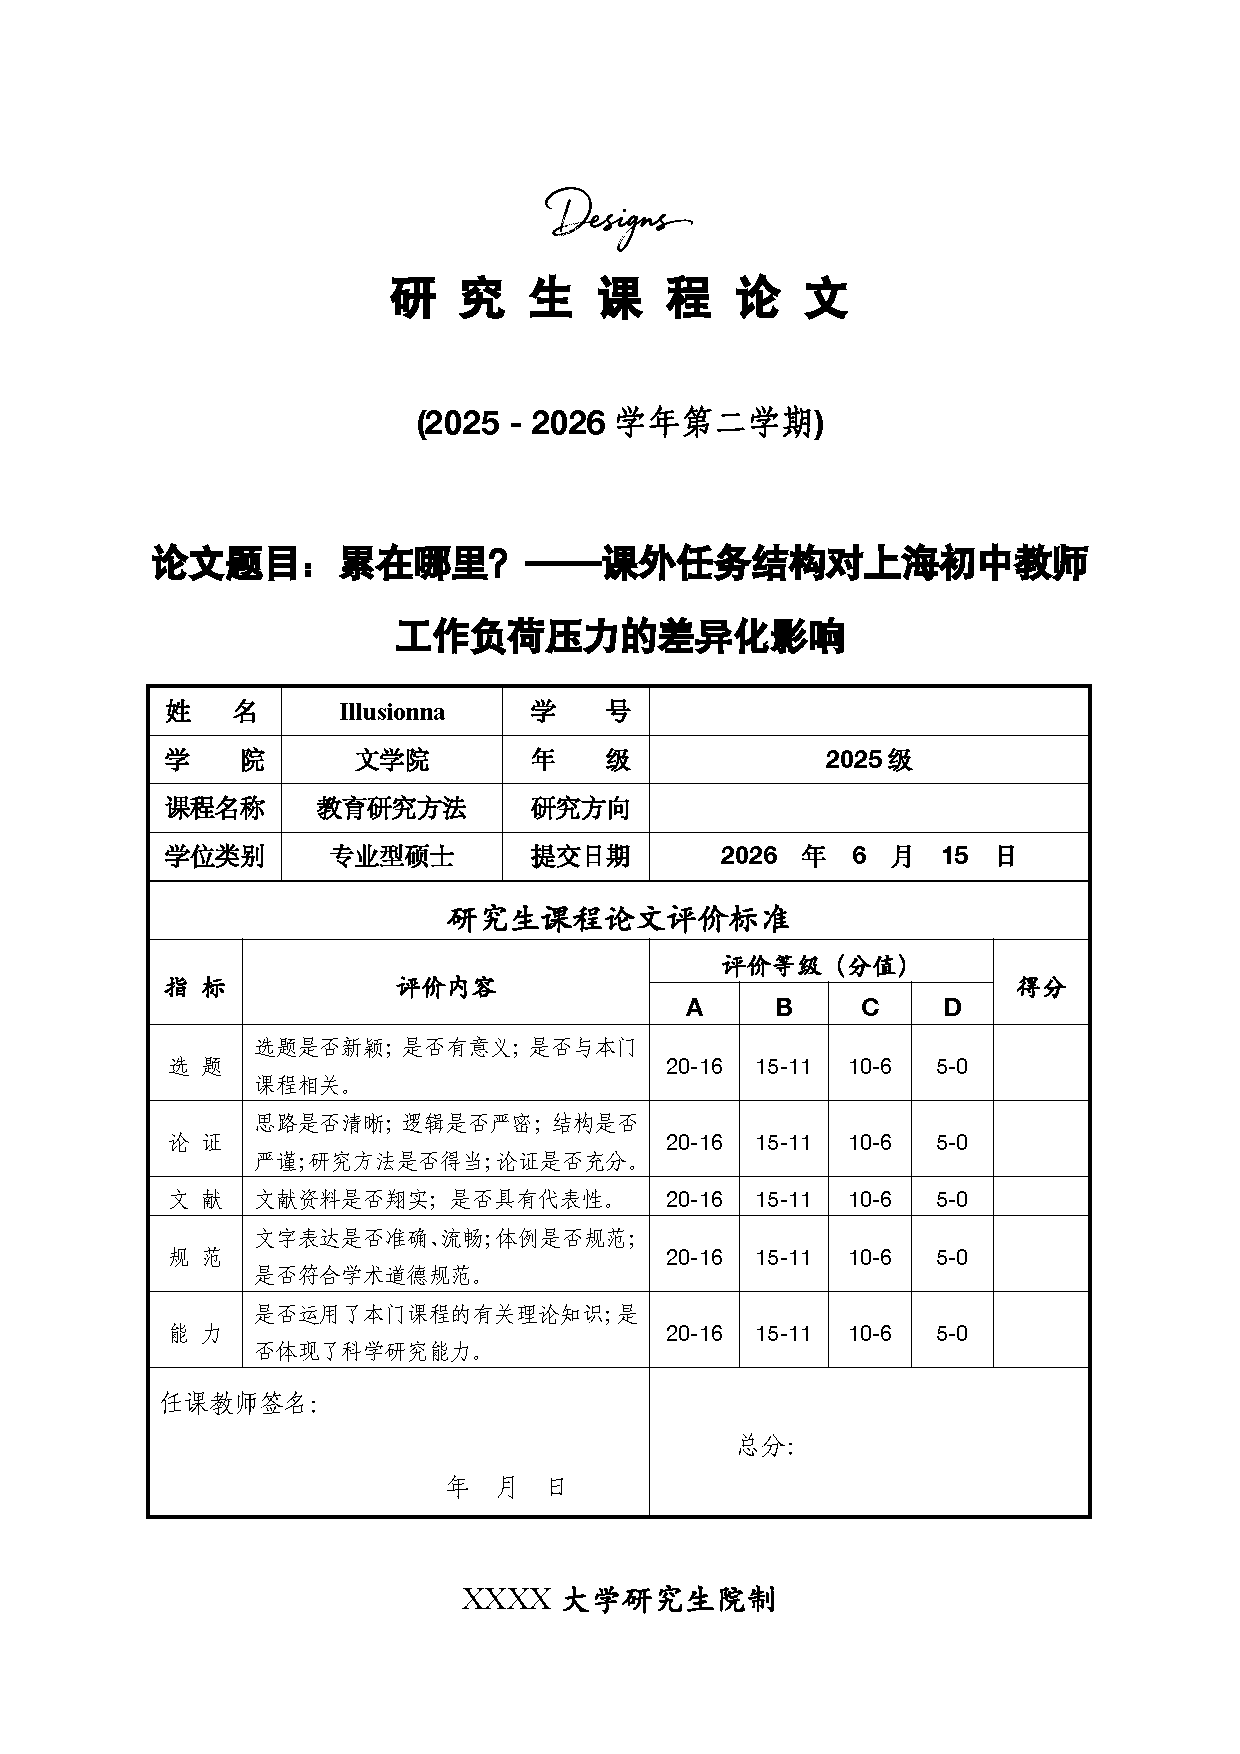
\includepdf[pages = -]{./figs/cover.pdf}
% \clearpage
% \thispagestyle{empty}
% \centerline{\tt12:05, Wednesday 31$^{\tt st}$ December, 2025 $\rightsquigarrow$ \currenttime,\ \today}
% \mbox{}
% \begin{spacing}{1.5}
%     \tableofcontents
% \end{spacing}
\clearpage
\vspace*{10em}

\centerline{\heiti\bfseries\zihao{2}研~究~生~课~程~论~文}
% \centerline{\heiti\bfseries\zihao{-3}（正文）}
\vspace*{4.2em}
% \centerline{\bfseries\zihao{-2}累在哪里？——课外任务结构对上海初中教师工作负荷压力的差异化影响}
\begin{center}
    \parbox{0.8\textwidth}{
    \centering\bfseries\zihao{-2}
        累在哪里？——课外任务结构对上海初中教师工作负荷压力的差异化影响
    }
\end{center}

\vspace*{1.8em}
\centerline{\bfseries\zihao{4}Illusionna}
\vspace*{3.2em}

\noindent\textbf{摘要：}教师“减负”政策通常默认行政性事务是教师负担的痛点，但该假设鲜有微观量化证据支撑，本次课程论文利用 OECD 教师教学国际调查 TALIS 2018 上海初中教师数据集（$N=3836$），在工作要求-资源模型 JD-R 框架下，综合运用分层加权最小二乘法回归、学校随机效应多层模型、分位数回归、调节效应分析与非参数 Bootstrap 推断，系统性探究九类课外任务对工作负荷压力的差异化影响。研究表明：批改作业是唯一强相关的任务类压力源（$\beta=0.219$），Bootstrap 95\% 置信区间为 $[0.175, 0.262]$，多层模型 $\beta=0.216$，批改时数最高四分位组的压力均值比最低组高 0.62 个标准差，而时数最多的备课并不致压，行政事务时数甚至与压力负相关。工作资源中，教师参与学校决策的保护效应最强（$\beta=-0.198,\ p<0.001$），且资源的纳入几乎不减弱批改作业的系数。负荷压力的学校间差异仅占 4.6\%（$\text{ICC}=0.046$），教师压力本质上是个体现象。分位数回归显示批改作业的致压效应随压力分位单调上升（$\beta_{0.1}=0.15,\ \beta_{0.7}=0.35$），其伤害集中于最“受不了”的教师群体。该效应存在性别差异，男教师批改时数更少（5.7 vs 8.4 小时/周），但单位时间致压效应更强（$\beta=0.29$ vs $\beta=0.198$），交互 $p=0.031$。本研究为“减什么”提供精确证据：作业批改治理与教师参与治理应优先于一般性的行政减负。

\vspace*{1em}

\noindent\textbf{关键词：}教师负担；TALIS 2018；工作负荷压力；批改作业



\clearpage
\chead{}
\cfoot{\thepage}
\setcounter{page}{1}



\section{引言}
教师工作负担过重一直是全球性议题，国内调查亦表明我国中小学教师工作量长期处于超负荷状态~\citep{LiXinCui}。2019 年中共中央办国务院办公厅印发印发《关于减轻中小学教师负担进一步营造教育教学良好环境的若干意见》~\citep{Education2019}，明确要求“把宁静还给学校，把时间还给教师”，2021 年“双减”政策实施后，课后服务的延展使中学教师在校时间被进一步拉长~\citep{Education2021}。在意见政策中，减负矛头直接指向“与教育教学无关的事项”——\textbf{填表}、\textbf{检查}、\textbf{评比}等行政性事务，其隐含的假设是，非教学负担是压垮教师的主要稻草，而教学本身的负担是教师的本职工作。

然而，教学负担的“时数”和“痛感”并不是一回事。同样一个小时，花在备课上和花在填表上，心理消耗未必相当，而被政策默认为“分内之事”的批改作业，反倒可能正是压力的大头。一旦减负瞄准的是那些时数不多、心理代价也不高的任务，政策的投入与教师真切的获得感之间，错位就难以避免。

为了厘清这种错位，我们需要能把课外各类任务的时间投入与教师主观的心理压力对应起来，形成细粒度微观数据。OECD 教师教学国际调查 TALIS 2018 轮次以上海作为我国的参测地区，提供了一套与国际接轨且记录完整的课外任务时间分配初中教师样本，为检验上述假设提供了理想的数据源支撑。据此，本文以上海初中教师为对象，研究以下三个递进式的问题：

\begin{itemize}
    \item 哪一类任务的时间投入才是工作负荷压力的真正预测源？
    \item 不同压力水平、不同教师群体中是否同质？
    \item 学校组织环境与教师拥有的工作资源能在多大程度上缓冲负担的影响？
\end{itemize}

不同于以往研究多采用的单一线性回归算法，本文的边际贡献在于提供完整的证据链：以分层回归识别平均效应，以多层模型分离学校与个体差异，以分位数回归刻画效应在教师压力分布上的异质性，以调节效应检验群体差异，最后以非参数 Bootstrap 对核心系数做不依赖分布假定的区间推断。这五类常规量化统计方法相互印证，构成对同一结论的多重检验。



\section{相关工作}
教师压力研究多年来都把工作要求—资源（JD-R）模型当作分析的骨架~\citep{BakkerDemerouti}。这个模型的思路，是把工作环境分成性质相反的两类：一类是工作要求，像工作量、时间压力、情绪付出，它们不断消耗精力，是倦怠最直接的来源；另一类是工作资源，比如自主性、来自同伴和领导的支持、专业发展与参与决策的机会，它们既能提升投入和满意度，又能在要求过高时充当缓冲，把损耗压下去。Kyriacou 对教师压力的经典界定~\citep{Kyriacou}，以及 OECD 近年提出的教师职业幸福感框架~\citep{Viac}，大体都可纳入这套要求—资源的二元结构。

JD-R 后来一个重要的细化，是把工作要求又分成挑战性要求和阻碍性要求两种。前者虽然也耗费精力，却常常伴随成长、掌控感和意义感，到头来能折算成专业上的回报；后者就是纯消耗，干完既不长本事，也说不上有什么成就。这个区分用到教师每天的活儿上，很说明问题。备课自主性高，与课堂表现和专业成长直接挂钩，更接近挑战性要求；批改作业则重复、机械、自主空间小、即时反馈又少，是阻碍性要求的典型；行政事务多被教师视作“与教学无关”的额外摊派；情绪劳动色彩浓重的家长沟通，同样难言成长。换言之，哪怕投入时间相同，不同任务在心理层面的“压力当量”也未必相等，这正是本文要检验的前提。

国内关于教师工作负担的讨论，我们可以大致可归为三类取向，回答的其实并非同一个问题。一类是对负担水平的测量与描述，李新翠~\citep{LiXinCui} 基于全国抽样调查发现，中小学教师的周工作量明显超出法定工时，且超出的部分越来越多地落在非教学事务和不易被看见的隐性劳动上，她由此主张有效调适而非一刀切地削减。第二类追问负担从何而来，质性研究指出~\citep{SongWu}，教师负担与其说是任务太多，不如说是行政发包、属地管理与层层问责沿科层链条传导、最终沉积到教师身上的制度产物，若真要减负，关键在切断这条生成链，而非在末端做减法。第三类则借助国际数据为本土经验定位，利用 TALIS 2018 描摹了上海教师教学实践的全球坐标~\citep{WangZhang}，发现教师在布置作业、批改与反馈上的投入强度位居参测经济体前列，这被视为上海经验的一部分，但背后教师付出的时间与心理代价，文中尚未在计量层面展开。

综合三条线索并置起来看，思辨与质性研究讲清了负担“从何而来”，描述性调查回答了负担“有多重”，唯独“哪一类负担最伤人”，即负担结构与教师主观心理痛感之间的量化关系，仍缺少基于代表性微观数据的系统检验，我的结课报告正是要补足这一环节。

值得注意的是，之所以选定上海，是因为它既典型又适合做这类检验，OECD 官方报告显示~\citep{OECD}，上海初中教师的周工作时间在全部参测经济体中名列前茅，其中批改作业的耗时约为国际均值的两倍——这与上海作业量大、又讲究全批全改的制度惯例直接相关~\citep{WangZhang}。但上海的情况并不只有“要求”这一面，当地教师投入教研与专业发展的时间同样远高于国际均值，且嵌在成熟的教研组制度之中，伴随着专业认同与同伴支持，再加上相对通畅的职称晋升通道与学校治理参与渠道，上海恰好提供了一个要求与资源都足够充分、可以同时检验二者效应的情境。



\section{研究假设与实验设计}
\subsection{假设}
\begin{itemize}
    \item[$\divideontimes$] \textbf{H1 政策话语假设：}相比备课、批改作业这类教学工作，学校管理、行政事务、家长沟通、组织课外活动等非教学任务花掉的时间，反而更容易让教师感到压力加重。
    \item[$\divideontimes$] \textbf{H2 任务属性假设：}决定压力大小的，关键在于这项任务本身是不是一种阻碍，而不在于它属不属于教学，正因如此，批改作业才会成为最突出的压力来源。
    \item[$\divideontimes$] \textbf{H3 资源保护假设：}工作资源，比如参与学校决策、师生关系、自我效能、同事合作等，负向预测压力，但不改变任务时数效应的相对格局。
    \item[$\divideontimes$] \textbf{H4 分布异质性假设：}教师批改作业的致压效应在压力分布的高分位段更强，即伤害集中于高压力教师。
\end{itemize}

\begin{figure}[H]
    \centering
    \begin{tikzpicture}[
        box/.style = {rounded corners = 3pt, align = center, font = \small, inner sep = 7pt, thick},
        lab/.style = {font = \footnotesize, fill = white, inner sep = 2pt},
        arr/.style = {-{Stealth[length = 2.6mm]}, thick, MorandiGrey}
    ]
        \node[box, draw = MorandiBlue, fill = MorandiBlue!12, text width = 4.6cm] (dem) {
            \textbf{工作要求}\footnotesize
            \\[4pt]
            九类课外任务周时数
            \\[2pt]
            （培训、行政、教研、备课、辅导、
            \\[2pt]
            批改、家长沟通、管理、课外活动）
        };

        \node[box, draw = MorandiPurple, fill = MorandiPurple!12, text width = 4.6cm, below = 1.1cm of dem] (res) {
            \textbf{工作资源}\footnotesize
            \\[4pt]
            同事交流合作 · 师生关系
            \\[2pt]
            自我效能感 · 参与学校决策
        };

        \node[box, draw = MorandiRed, fill = MorandiRed!12, text width = 3.6cm, right = 3.6cm of $(dem.east)!0.5!(res.east)$] (out) {
            \textbf{工作负荷压力}\footnotesize
            \\[4pt]
            T3WLOAD
            \\[2pt]
            （稳定性：T3WELS）
        };

        \node[box, draw = MorandiOrange, fill = MorandiOrange!25, above = 1cm of out, text width = 3.6cm] (mod) {
            \footnotesize\textbf{调节变量：}教龄 · 性别
        };

        \draw[arr] (dem.east) -- node[lab, pos = 0.45] {H1 / H2（$+$）} (out.150);
        \draw[arr] (res.east) -- node[lab, pos = 0.45] {H3（$-$）} (out.210);
        \draw[arr, dashed, MorandiOrange!80!black] (mod.south) -- (out.north);

        \node[below = 0.4cm of out, text width = 4.2cm, align = center, font = \footnotesize, color = MorandiGrey] {
            H4：效应沿压力分布变化
            \\[2pt]
            （分位数回归）
        };
        \node[below = 0.4cm of res, font = \footnotesize, color = MorandiGrey, text width = 4.8cm, align = center] {
            控制：学历、性别、教龄
            \\[2pt]
            学校层差异：随机截距多层模型
        };
    \end{tikzpicture}
    \caption{研究的分析框架 JD-R 模型}\label{JD-R}
\end{figure}

图~\ref{JD-R} 汇总了整个分析框架：九类任务时数构成工作要求，四个量表构成工作资源，二者共同预测压力；性别与教龄作为调节变量进入模型；学校层面的差异交由多层模型分离，效应在压力分布上的异质性则由分位数回归刻画。



\subsection{数据集}
数据取自 OECD 官网公开的 TALIS 2018 数据库，使用的是初中教师问卷部分，其中上海子样本规模为 198 所初中、3976 名教师~\footnote{\href{https://www.kaggle.com/datasets/illusionna/oecd-talis-2018}{https://www.kaggle.com/datasets/Illusionna/oecd-talis-2018}}，抽样分两个阶段：先抽学校，再到校内随机抽教师，并按学校类型分层。我们剔除关键变量缺失的个例，最终用于分析的样本为 $N=3836$，除非另作说明，后续所有估计都按教师最终权重 TCHWGT 进行加权。



\subsection{变量阐述}
因变量为 TALIS 官方量表工作负荷压力指数 T3WLOAD，稳定性检验采用职业幸福与压力指数 T3WELS，两者均经验证性因子分析合成，取值越高压力越大。工作要求为九类课外任务的周时数 TT3G18A-I，经 1\%/99\% 分位数缩尾处理以抑制极端值，工作资源为四个官方量表，包含师生关系 T3STUD、自我效能感 T3SELF、参与学校决策 T3STAKE 与同事交流合作 T3EXCH。控制变量为性别、学历（硕士及以上）与教龄。表~\ref{description} 报告展示了加权描述统计。

\begin{table}[H]
    \centering
    \caption{主要变量加权描述统计（$N=3836$）}\label{description}
    \setlength{\tabcolsep}{8pt}
    \renewcommand{\arraystretch}{1.5}
    \begin{threeparttable}
        \begin{tabular}{clcccc}
            \bottomrule[1.5pt]
            ~ & \multicolumn{1}{c}{\textbf{变量}} & \textbf{类别} & \textbf{加权均值} & \textbf{标准差} & \textbf{与压力相关 $r$} \\
            \midrule[0.5pt]
            \cube{MorandiBlue} & 个人备课（h/周） & 教学性 & 8.44 & 6.47 & $0.101$ \\
            \rowcolor{MorandiLightCyan}
            \cube{MorandiBlue} & 批改作业（h/周） & 教学性 & 7.64 & 5.87 & $\mathbf{0.250}$ \\
            \cube{MorandiCyan} & 学生辅导咨询（h/周） & 育人性 & 5.10 & 4.35 & $0.138$ \\
            \cube{MorandiCyan} & 团队协作与教研（h/周） & 专业性 & 3.94 & 3.24 & $0.016$ \\
            \cube{MorandiCyan} & 专业发展活动（h/周） & 专业性 & 3.13 & 3.03 & $-0.011$ \\
            \cube{MorandiRed} & 参与学校管理（h/周） & 非教学 & 3.15 & 5.79 & $-0.046$ \\
            \cube{MorandiRed} & 一般行政事务（h/周） & 非教学 & 2.77 & 4.76 & $-0.095$ \\
            \cube{MorandiRed} & 家长沟通（h/周） & 非教学 & 2.08 & 2.12 & $0.098$ \\
            \cube{MorandiRed} & 课外活动（h/周） & 非教学 & 1.78 & 2.20 & $0.012$ \\
            \midrule[0.5pt]
            \cube{MorandiPurple} & 参与学校决策 & 资源 & 11.23 & 2.49 & $-0.213$ \\
            \cube{MorandiPurple} & 师生关系 & 资源 & 13.27 & 2.39 & $-0.090$ \\
            \cube{MorandiPurple} & 自我效能感 & 资源 & 12.67 & 2.71 & $-0.028$ \\
            \cube{MorandiPurple} & 同事交流合作 & 资源 & 10.98 & 2.10 & $0.009$ \\
            \midrule[0.5pt]
            \cube{MorandiGrey} & 工作负荷压力（T3WLOAD） & 因变量 & 9.18 & 1.98 & - \\
            \cube{MorandiGrey} & 职业幸福与压力（T3WELS） & 因变量 & 9.34 & 1.82 & $0.515$ \\
            \toprule[1.5pt]
        \end{tabular}

        \begin{tablenotes}\small
            \item 【注】TCHWGT 加权，时数变量经 1\%/99\% 缩尾，$r$ 为与工作负荷压力的 Pearson 相关
        \end{tablenotes}
    \end{threeparttable}
\end{table}



\subsection{计量模型}
\subsubsection{基准模型}
记教师 $i$ 的压力为标量 $y_i$，九类任务时数为标量 $h_{k,i}$，其中 $k=1,2,\ldots,9$，工作资源为标量 $r_{m,i}$，其中 $m=1,2,3,4$，控制变量向量为 $\bm{x}_i\in\mathbb{R}^{3}$，对应系数向量为 $\bm{\delta}\in\mathbb{R}^{3}$，基准设定为：
\begin{align}
    y_i=\alpha+\sum_{k=1}^{9}\beta_k h_{k,i}+\sum_{m=1}^{4}\gamma_m r_{m,i}+\bm{\delta}^{\top}\bm{x}_i+\varepsilon_i
\end{align}

其中 $\alpha,\beta_k,\gamma_m$ 为标量系数，$\varepsilon_i$ 为标量误差项，连续变量均经 $z$ 变换标准化，故 $\beta_k$ 为标准化系数，可直接比较相对大小，M1、M2、M3 按“控制变量 $\rightarrow$ 加入工作要求 $\rightarrow$ 加入工作资源”分层录入。

将全部回归元堆叠为向量 $\bm{z}_i=(1,h_{1,i},\ldots,h_{9,i},r_{1,i},\ldots,r_{4,i},\bm{x}_i^{\top})^{\top}\in\mathbb{R}^{17}$，对应完整系数向量 $\bm{\beta}=(\alpha,\beta_1,\ldots,\beta_9,\gamma_1,\ldots,\gamma_4,\bm{\delta}^{\top})^{\top}\in\mathbb{R}^{17}$，模型遂可紧凑写成：
\begin{align}
    y_i=\bm{z}_i^{\top}\bm{\beta}+\varepsilon_i
\end{align}

再令响应向量 $\bm{y}=(y_1,\ldots,y_n)^{\top}\in\mathbb{R}^{n}$，设计矩阵 $\bm{Z}=(\bm{z}_1,\ldots,\bm{z}_n)^{\top}\in\mathbb{R}^{n\times 17}$，权重矩阵 $\bm{W}=\operatorname{diag}(\omega_1,\ldots,\omega_n)\in\mathbb{R}^{n\times n}$，即：
\begin{align}
    \bm{W}=\begin{pmatrix}
        \omega_1 & 0 & \cdots & 0 \\
        0 & \omega_2 & \cdots & 0 \\
        \vdots & \vdots & \ddots & \vdots \\
        0 & 0 & \cdots & \omega_n
    \end{pmatrix}
\end{align}

考虑抽样设计，参数以加权最小二乘 WLS 估计：
\begin{align}
    \hat{\bm{\beta}}=\arg\min_{\bm{\beta}}\sum_{i=1}^{n}\omega_i\bigl(y_i-\bm{z}_i^{\top}\bm{\beta}\bigr)^2=\bigl(\bm{Z}^{\top}\bm{W}\bm{Z}\bigr)^{-1}\bm{Z}^{\top}\bm{W}\bm{y}
\end{align}

其中 $\omega_i$ 为 TCHWGT 权重，标准误采用异方差稳健的 HC1 三明治估计。



\subsubsection{多层模型}
教师嵌套于学校，记教师 $i$ 属于学校 $j$，即 $i\in j$，令 $\bm{z}_{ij}\in\mathbb{R}^{17-1}$ 为教师 $i$ 的层一协变量向量，即除常数项外的全部回归元，$\bm{\beta}$ 为对应固定效应系数向量，以随机截距模型分离两层变异：
\begin{align}
    y_{ij}=\gamma_{00}+\bm{z}_{ij}^{\top}\bm{\beta}+u_j+\varepsilon_{ij}\qquad u_j\sim N(0,\sigma_u^2)\qquad\varepsilon_{ij}\sim N(0,\sigma_\varepsilon^2)
\end{align}

其中 $\gamma_{00}$ 为总截距，$u_j$ 为学校层随机截距，$\varepsilon_{ij}$ 为个体层残差，三者均为标量，且 $u_j$ 与 $\varepsilon_{ij}$ 相互独立，学校间变异占比由组内相关系数 ICC 度量：
\begin{align}
    \mathrm{ICC}=\dfrac{\sigma_u^2}{\sigma_u^2+\sigma_\varepsilon^2}
\end{align}



\subsubsection{分位数回归}
与刻画条件均值不同，分位数回归~\citep{Koenker} 估计压力条件分布第 $\tau$ 分位处的效应：
\begin{align}
    \hat{\bm{\beta}}(\tau)=\arg\min_{\bm{\beta}}\sum_{i=1}^{n}\rho_{\tau}\left(y_i - \bm{z}_i^{\top}\bm{\beta}\right)\qquad \rho_{\tau}(u)=u\bigl(\tau-\mathbb{I}\{u<0\}\bigr)
\end{align}

其中 $\bm{z}_i$ 与 $\bm{\beta}$ 沿用回归元与系数向量，$\tau\in(0,1)$ 为分位水平，$\rho_{\tau}(\cdot)$ 为非对称绝对值损失，其自变量 $u$ 与示性函数 $\mathbb{I}\{\cdot\}$ 均为标量，标量分量 $\beta_{\text{批改}}(\tau)$ 随 $\tau$ 的轨迹回答“批改作业对谁的伤害更大”。



\subsubsection{调节效应}
加入乘积项检验群体异质性，以性别为例：
\begin{align}
    y_i=\alpha+\beta_Ch_{C,i}+\theta\left(h_{C,i}\times\mathrm{female}_i\right)+\cdots+\varepsilon_i
\end{align}

其中 $h_{C,i}$ 为教师 $i$ 的批改作业时数，$\mathrm{female}_i\in\{0,1\}$ 为性别示性变量，$\beta_C,\theta$ 为标量系数，$\theta$ 显著即表明批改作业的边际效应因性别而异，男、女教师的斜率分别为 $\beta_C$ 与 $\beta_C+\theta$。



\subsubsection{Bootstrap 推断}
为避免区间推断依赖正态性假定，以非参数 Bootstrap 重抽样，有放回抽取 $n$ 个个体并重估，重复 $B=1000$ 次。对任一标量系数 $\beta_j$，记第 $b$ 轮重估值为 $\hat\beta_j^{*(b)}$，其中 $b=1,2,\ldots,B$，得其经验抽样分布 $\{\hat\beta_j^{*(1)},\dots,\hat\beta_j^{*(B)}\}$，令 $\hat\beta_{j,(r)}^{*}$ 为该分布由小到大的第 $r$ 个次序统计量，按百分位法构造置信区间：
\begin{align}
    \mathrm{CI}_{95\%}(\beta_j)=\left[\hat\beta_{j,(\lfloor 0.025B\rfloor)}^{*},\ \hat\beta_{j,(\lceil 0.975B\rceil)}^{*}\right]
\end{align}

关于模型解释力需要事先说明，压力类心理结果的个体差异主要由人格特质、健康状况、家庭事件等问卷未测因素驱动，横截面问卷研究的 $R^2$ 通常在 $0.05\sim0.25$ 之间，按效应量基准~\citep{Cohen}：
\begin{align}
    f^2=\dfrac{R^2}{1-R^2}
\end{align}

已属小至中等效应，因此本文的评价重点放在标准化系数的相对大小与跨模型稳定性，而非追求高拟合优度。



\subsection{实验环境与依赖}
表~\ref{dependency} 展示了本次实验所用到的数据处理、统计估计与图表制作等所有依赖环境，以 pyreadstat 读取 OECD 发布的 SPSS 数据文件，pandas/numpy 完成清洗与变换，再用 statsmodels 完成 WLS、多层模型与分位数回归估计，matplotlib/seaborn 输出图像，Xe\LaTeXe 排版论文，随机过程 Bootstrap 重抽样、散点抽样展示等，均固定 NumPy PCG64 随机数种子 seed 为 42。

\begin{table}[H]
    \centering
    \caption{实验环境依赖}\label{dependency}
    \setlength{\tabcolsep}{15pt}
    \renewcommand{\arraystretch}{1.5}
    \begin{tabular}{cll}
        \bottomrule[1.5pt]
        ~ & \multicolumn{1}{c}{\textbf{组件}} & \multicolumn{1}{c}{\textbf{版本 / 配置}} \\
        \midrule[0.5pt]
        \cube{MorandiGrey} & 硬件平台 & Apple M2（arm64） \\
        \cube{MorandiGrey} & 操作系统 & macOS Sonoma 14.6（Build 23G80） \\
        \cube{MorandiGrey} & 编译工具链 & clang 16.0.0 Arm64-Apple-Darwin23.6.0 (posix) \\
        \midrule[0.5pt]
        \cube{MorandiBlue} & Python & 3.12.0（独立 Miniconda 环境） \\
        \cube{MorandiBlue} & 数值与数据处理 & numpy 2.2.0、pandas 2.3.3、scipy 1.16.3 \\
        \cube{MorandiBlue} & 统计建模 & statsmodels 0.14.6（WLS / MixedLM / QuantReg） \\
        \cube{MorandiBlue} & 数据读取 & pyreadstat 1.3.5（SPSS *.sav 及元数据） \\
        \cube{MorandiBlue} & 可视化 & matplotlib 3.10.0、seaborn 0.13.2 \\
        \midrule[0.5pt]
        \cube{MorandiCyan} & 排版引擎 & XeTeX 3.141592653-2.6-0.999996（TeX Live 2024） \\
        \cube{MorandiCyan} & 随机数 & NumPy PCG64、种子 42、Bootstrap $B=1000$ \\
        \toprule[1.5pt]
    \end{tabular}
\end{table}



\subsection{实验流程}
图~\ref{process} 给出从数据获取到结论的完整量化分析流程，整体上对应 4 个环节：预处理环节数据标准化与加权、模型估计环节依次执行四类估计、稳定性环节以替换因变量、Bootstrap 重抽样与效应量评价共同确认结论。

\begin{figure}[H]
    \centering
    \begin{tikzpicture}[
        stage/.style = {
            rounded corners = 3.5pt,
            align = left,
            inner xsep = 12pt,
            inner ysep = 7pt,
            text width = 12.6cm,
            thick
        },
        sarr/.style = {
            -{Stealth[length = 2.8mm]},
            very thick,
            MorandiGrey!75
        },
        node distance = 0.5cm
    ]
        \node[stage, draw = MorandiGrey!75, fill = MorandiGrey!8] (s1) {
            \textbf{\textcolor{MorandiGrey}{①~数据获取}}\footnotesize\quad
            OECD TALIS 2018 公开数据库，上海初中教师问卷（198 所学校、$N=3976$），pyreadstat 读取 SPSS 数据及变量元信息
        };

        \node[stage, draw = MorandiBlue!75, fill = MorandiBlue!8, below = of s1] (s2) {
            \textbf{\textcolor{MorandiBlue}{②~数据预处理}}\footnotesize\quad
            剔除关键变量缺失（$N:\ 3976\to3836$）、任务时数 1\%/99\% 缩尾、连续变量 $z$ 标准化、TCHWGT 抽样权重
        };

        \node[stage, draw = MorandiCyan!85, fill = MorandiCyan!10, below = of s2] (s3) {
            \textbf{\textcolor{MorandiCyan!70!black}{③~描述性分析}}\footnotesize\quad
            加权描述统计、时间结构玫瑰图、气泡相关矩阵、分组云雨图
        };

        \node[stage, draw = MorandiPurple!75, fill = MorandiPurple!8, below = of s3] (s4) {
            \textbf{\textcolor{MorandiPurple}{④~模型估计}}\footnotesize\quad
            分层 WLS + HC1 稳健标准误（M1$\to$M3）、学校随机截距多层模型与 ICC、分位数回归（$\tau=0.1\sim0.9$）、性别 $\times$ 批改调节效应
        };

        \node[stage, draw = MorandiRed!80, fill = MorandiRed!8, below = of s4] (s5) {
            \textbf{\textcolor{MorandiPurple}{⑤~稳定性与推断}}\footnotesize\quad
            替换因变量 T3WELS（M5）、Bootstrap $B=1000$ 百分位区间、效应量 $f^2$ 与 $\Delta R^2$ 评价 $\Rightarrow$ 结论与政策建议
        };

        \draw[sarr] (s1) -- (s2);
        \draw[sarr] (s2) -- (s3);
        \draw[sarr] (s3) -- (s4);
        \draw[sarr] (s4) -- (s5);
    \end{tikzpicture}
    \caption{量化分析流程}\label{process}
\end{figure}



\section{实证结果}
\subsection{教师时间支配情形}
上海初中教师每周总工作时间 45.3 小时，课外任务合计 38.1 小时，图~\ref{rose} 直观呈现其结构，花瓣面积随时数递减顺时针展开，最大的两瓣——备课 8.4 h 与批改 7.6 h 均为教学性任务，合计 16.1 小时，占 42.3\%，专业与育人性任务 12.2 小时，占 32.0\%，被政策话语重点关注的非教学性任务四瓣合计仅 9.8 小时，占 25.7\%，因此，“教师时间被行政杂务大量挤占”的叙事在时数层面即不成立。

图~\ref{bubble} 是 Pearson 相关系数矩阵，可以给出初步线索，九类时数中批改作业与压力的相关最强（$r=0.25$），资源变量中参与学校决策与压力的负相关最强（$r=-0.21$），各任务时数之间相关普遍较弱，最强的一对的学校管理与行政事务（$r=0.59$）亦远低于共线警戒水平。

在正式回归之前，不妨先看图~\ref{raincloud}，它不带任何模型假定，直接把核心关系摆出来。把教师按批改时数分成四组，可以看到压力的核密度“云”、底下的数据点“雨”连同四分位距，整体都在往右挪：加权均值从 Q1 组（每周不超过 3 小时）的 8.48，一路升到 Q4 组（每周 10 小时以上）的 9.70，两头差出 1.22 个原始分，折合约 0.62 个标准差。这样一条剂量—反应式的梯度，在动用任何模型之前就已经摆在那里——后面回归得出的结论之所以稳，直观的底气也正在于此。

\begin{figure}[H]
    \centering
    \includegraphics*[width=0.75\textwidth]{./figs/rose.pdf}
    \caption{上海初中教师每周任务时间加权均值分布（$\text{花瓣半径}\propto\sqrt{\text{时数}}$）}\label{rose}
\end{figure}

\begin{figure}[H]
    \centering
    \includegraphics*[width=0.85\textwidth]{./figs/bubble.pdf}
    \caption{下三角相关系数矩阵（$\text{气泡面积}\propto|r|$ 且仅标注 $|r|\geqslant0.18$ 的系数）}\label{bubble}
\end{figure}

\begin{figure}[H]
    \centering
    \includegraphics*[width=0.89\textwidth]{./figs/raincloud.pdf}
    \caption{批改作业时数四分位压力分布（上为加权核密度、下随机抽样 260 人/组的点列）}\label{raincloud}
\end{figure}



\subsection{基准回归、多层模型与 Bootstrap 的批改作业情形}
表~\ref{regression} 是 ICC 的估计结果，M2 中，批改作业是唯一强正向的任务 $\beta=0.233$、$p<0.001$，加入资源后的 M3 中其系数仅微降至 0.219，几乎不被资源吸收，即 H3 成立，学校随机截距的 M4 中为 0.216，依旧显著。与之对照的是，备课在全部模型中不显著，行政事务稳定为负，在 M3 中 $\beta=-0.086$、$p<0.001$，图~\ref{forest} 的系数直观显示 M2 与 M3 的估计几乎重合，任务时数的效应格局对资源的纳入完全稳健。

\begin{figure}[H]
    \centering
    \includegraphics*[width=0.89\textwidth]{./figs/forest.pdf}
    \caption{九类任务时数的系数对比 M2（仅要求）与 M3（要求和资源）几乎重合}\label{forest}
\end{figure}

\begin{table}[H]
    \centering
    \caption{课外任务时数与工作资源对教师压力的回归（标准化系数）}\label{regression}
    \setlength{\tabcolsep}{4pt}
    \renewcommand{\arraystretch}{1.5}
    \begin{threeparttable}
        \begin{tabular}{clccccc}
            \bottomrule[1.5pt]
            ~ & \multicolumn{1}{c}{\textbf{变量}} & \textbf{M1} & \textbf{M2} & \textbf{M3} & \textbf{M4 多层} & \textbf{M5 (T3WELS)} \\
            \midrule[0.5pt]
            ~ & \multicolumn{1}{c}{女性} & $-0.054$ & $-0.172^{***}$ & $-0.164^{***}$ & $-0.173^{***}$ & $-0.094^{*}$ \\
            ~ & \multicolumn{1}{c}{硕士及以上} & $0.065$ & $0.052$ & $0.054$ & $0.054$ & $-0.109^{*}$ \\
            ~ & \multicolumn{1}{c}{教龄} & $0.040^{*}$ & $0.029$ & $0.025$ & $0.026$ & $0.051^{**}$ \\
            \midrule[0.5pt]
            \cube{MorandiBlue} & 个人备课 & & $0.029$ & $0.028$ & $0.035^{*}$ & $0.009$ \\
            \rowcolor{MorandiLightCyan}
            \cube{MorandiBlue} & 批改作业 & & $\mathbf{0.233^{***}}$ & $\mathbf{0.219^{***}}$ & $\mathbf{0.216^{***}}$ & $\mathbf{0.128^{***}}$ \\
            \cube{MorandiCyan} & 团队协作与教研 & & $-0.041^{*}$ & $-0.040$ & $-0.034$ & $-0.021$ \\
            \cube{MorandiCyan} & 专业发展活动 & & $-0.034$ & $-0.031$ & $-0.044^{*}$ & $-0.057^{**}$ \\
            \cube{MorandiCyan} & 学生辅导咨询 & & $0.045^{*}$ & $0.046^{*}$ & $0.042^{*}$ & $0.049^{*}$ \\
            \cube{MorandiRed} & 参与学校管理 & & $0.000$ & $0.014$ & $0.005$ & $0.069^{**}$ \\
            \cube{MorandiRed} & 一般行政事务 & & $-0.092^{***}$ & $-0.086^{***}$ & $-0.075^{***}$ & $-0.034$ \\
            \cube{MorandiRed} & 家长沟通 & & $0.018$ & $0.016$ & $0.016$ & $0.073^{***}$ \\
            \cube{MorandiRed} & 课外活动 & & $0.024$ & $0.033$ & $0.040^{*}$ & $-0.041^{*}$ \\
            \midrule[0.5pt]
            \cube{MorandiPurple} & 参与学校决策 & & & $-0.198^{***}$ & $-0.205^{***}$ & $-0.249^{***}$ \\
            \cube{MorandiPurple} & 师生关系 & & & $0.018$ & $0.014$ & $-0.016$ \\
            \cube{MorandiPurple} & 自我效能感 & & & $-0.007$ & $0.007$ & $-0.042^{*}$ \\
            \cube{MorandiPurple} & 同事交流合作 & & & $0.026$ & $0.038^{*}$ & $0.027$ \\
            \midrule[0.5pt]
            ~ & $R^2$ & 0.002 & 0.081 & 0.116 & ICC$=0.046$ & 0.123 \\
            ~ & $N$ & 3\,836 & 3\,836 & 3\,836 & 3\,836 & 3\,836 \\
            \toprule[1.5pt]
        \end{tabular}

        \begin{tablenotes}\small
            \item 【注】$^{*}p<0.05$、$^{**}p<0.01$、$^{***}p<0.001$，M1、M2、M3、M5 为 WLS，即 TCHWGT 加权 HC1 稳健标准误，M4 为学校随机截距多层模型，即 REML 未加权，M5 因变量为职业幸福与压力指数
        \end{tablenotes}
    \end{threeparttable}
\end{table}

按照非参数 Bootstrap（$B=1000$）进一步给出不依赖正态假定的推断，图~\ref{boot} 将九类任务系数的全部抽样分布绘成脊线图，可以看出，批改作业的整个分布孤悬于零线右侧远处，95\% 百分位区间 $[0.175, 0.262]$ 与零相距 8 个以上标准误，行政事务的分布则完整落在零线左侧（$[-0.13, -0.05]$），其余七类任务的分布均横跨零线。系数的不确定性被完整可视化之后，“批改独大”的格局一目了然。

资源侧的发现同样重要，参与学校决策是最强保护因素，其 M3 达到 $\beta=-0.198$，M5 为 $\beta=-0.249$，均 $p<0.001$，其效应量与批改作业相当而方向相反。师生关系、自我效能与同事交流则在控制其他变量后基本不显著。这提示压力管理的杠杆不在个体心理建设，而在治理结构中，教师对学校事务是否拥有发言权。ICC 计算仅为 0.046，压力的学校间差异不足 5\%，教师压力本质上是个体层现象，仅靠选择好学校无法回避，干预需落到任务与个体层面。

\begin{figure}[H]
    \centering
    \includegraphics*[width=0.9\textwidth]{./figs/boot.pdf}
    \caption{九类任务系数的 Bootstrap 抽样分布（横线为 95\% 百分位区间、圆点为中位数）}\label{boot}
\end{figure}



\subsection{伤害集中于高压力教师情形}
均值回归可能掩盖效应在分布两端的差异，图~\ref{qheat} 将九类任务在 $\tau=0.1\to0.9$ 上的全部分位数系数绘成热图。

\begin{figure}[H]
    \centering
    \includegraphics*[width=0.95\textwidth]{./figs/qheat.pdf}
    \caption{九类任务时数的分位数回归系数}\label{qheat}
\end{figure}

这一点看图最清楚，批改作业那一行用蓝框圈出来，颜色自左向右一格深过一格，系数从 $\beta_{0.1}=0.15$ 起步，爬到 $\beta_{0.7}=0.35$ 见顶，高分位段约为低分位段的 2.3 倍。更关键的是，9 个分位点全部在 0.1\% 水平上显著，这种“全程亮着”的行，整张图里仅此 1 条，反观行政事务那一行，始终是浅蓝的负值，其中几个分位点显著为负。两相对照说明：只看均值、搞“普惠式”减负，其实低估真正能兑现的收益，压力越大、越接近崩溃边缘的教师，从作业批改治理中得到的回报越高，靶向性相当突出。H4 由此得到支持。



\subsection{男教师暴露更少痛感更强的异质情形}
图~\ref{radar} 先呈现两性的时间画像，女教师在批改作业上的投入为 8.4 h/周，远高于男教师的 5.7 h/周，备课、辅导与家长沟通亦更高，而男教师仅在学校管理、行政与课外活动上略多，两性负担的东西并不相同。

\begin{figure}[H]
    \centering
    \includegraphics*[width=0.75\textwidth]{./figs/radar.pdf}
    \caption{男女教师每周课外任务时间画像（加权均值为 h/周）}\label{radar}
\end{figure}

调节效应的结果有点出乎意料，男教师批改量更少，但单位时间内的致压效应反而更强，交互项 $\hat\theta=-0.094$、$p=0.031$，图~\ref{sex} 把这种反差画了出来，其中实线是预测值，阴影为 95\% 置信带，灰点是随机抽取的 900 名教师。对比两条线可以看到，男教师的斜率 $\beta=0.292$ 明显比女教师 $\beta=0.198$ 更陡。

\begin{figure}[H]
    \centering
    \includegraphics*[width=0.9\textwidth]{./figs/sex.pdf}
    \caption{按性别的批改作业时数与预测压力}\label{sex}
\end{figure}

暴露少而痛感强的组合更支持教师职业期望落差解释，批改在男教师的职业自我认知中更可能被归类为低回报的事务性劳动，也可能与其承担的班主任、竞赛辅导等并行角色的时间挤压有关，具体机制有待后续研究。另一方面，批改作业与教龄分组（新手和资深）的交互不显著（$p=0.78$），批改的致压效应不随经验积累而消退，因此诸如“熬过新手期就好了”的言论并不成立。



\subsection{效应量评价情形}
显著只是第一步，要真正解读结果还得回到效应量。以批改作业为例，$\beta=0.219$ 的意思是：批改时数每增加一个标准差（约每周 5.9 小时），压力上升 0.219 个标准差，这个数字也不是孤证，图~\ref{raincloud} 中 Q4 组与 Q1 组的均值相差 0.62 个标准差，与它对得上。横截面数据里，压力这类心理变量本来就很难有大效应，所以这个量级算是相当强的任务效应了，也是九类任务中唯一一个稳稳站上 0.2 的。

其次，全模型 $R^2=0.116$ 对应 $f^2 = \dfrac{R^2}{1-R^2}=0.13$，按基准~\citep{Cohen} 接近中等效应，考虑到压力的个体差异主要由人格、健康等问卷外因素决定，任务时数模块独立贡献的 $\Delta R^2=0.079$ 已具实质意义。

而且更重要的是体系的稳定性，批改作业的系数在全部模型设定（M2、M3、M4、M5、九个分位点及 1000 次 Bootstrap 重抽样）中方向一致，并且始终显著，但备选解释（备课、行政）在任何设定下都不成立，即结论的可信度来自多重检验的一致性，而非单一模型的拟合优度。



\section{结论与探讨}
回到开篇的疑问——压垮上海初中教师的是不是那些被政策反复点名的填表、检查与评比？五类方法给出的答案出奇一致，并不是。每周三十八小时的课外投入里，行政、管理等非教学事务占去的还不到十小时，谈不上“挤占”，其时数甚至与压力稳定地负相关。“行政杂务压垮教师”的流行叙事，在时间投入与心理代价两个层面同时落了空，H1 被否证。这并非说行政摊派不值得治理，而是若把减负的力气几乎都压在这一头，瞄准的恰恰是时数与心理当量都不高的那部分，引言所担心的政策投入与教师获得感之间的错位，便实实在在地发生了。

真正的压力源是批改作业。它是九类任务中唯一在所有设定下都站得住脚的强预测源——分层 WLS、分离学校层差异的多层模型、分位数回归与不依赖正态假定的 Bootstrap 区间，系数始终为正且显著，换用另一套量表 T3WELS 重做亦然。结论的可信度正来自这种跨模型、跨指标的一致性，而非某个模型碰巧拟合得好。与之对照，耗时最多的备课却始终不致压：备课自主性高、与专业成长直接挂钩，更像带来掌控感的挑战性要求，而批改重复机械、反馈又少，是阻碍性要求的典型。

可见决定痛感的不是“教不教学”，也不是花了多少时间，而是任务的属性，H2 得到支持。这份伤害还并不均匀，分位数回归显示其致压效应随压力分位单调抬升，对最“受不了”的教师接近低分位段的两倍多，即 H4 成立，意味着以均值为靶的“普惠式”减负低估了收益。性别上则呈现“暴露更少、痛感更强”的反差：女教师批改投入远多于男教师，但男教师单位时间的致压效应反而更强，或可用职业期望落差解释，确切机制有待后续追究；而批改与教龄交互不显著，说明这份压力不随经验消退。

资源一侧，四个工作资源里唯有参与学校决策具有与批改相当、方向相反的保护效应，个体心理资源几乎不起作用。纳入资源后批改系数纹丝不动，资源能缓冲压力却改不了任务的相对格局，H3 成立。加之 ICC 仅 0.046，学校间差异不足 5\%，教师压力本质上是个体现象，靠“挑一所好学校”难以回避。据此我们提三点建议：

\begin{itemize}
    \item[$\bigstar$] 减负的着力点应从“压缩行政”转向“作业批改”治理，控制作业总量、推行分层作业与抽样批改、审慎引入 AI 技术辅助，把省下的时间转化为更有回报的反馈设计。
    \item[$\bigstar$] 扩大教师参与式治理，给教师对学校事务的发言权是成本极低的组织性减压手段。
    \item[$\bigstar$] 有限资源应向高压力群体投放，优先为带班多批改量大的教师配置作业管理支持。
\end{itemize}



\clearpage
\cfoot{}
\setlength{\bibhang}{2em}
\renewcommand{\refname}{}
\centerline{\zihao{3}\bfseries\@参考文献}
\vspace*{-3em}

\begin{thebibliography}{16}\zihao{5}
    \bibitem[教育部(2019)]{Education2019} 教育部. (2019). 中共中央办公厅, 国务院办公厅印发《关于减轻中小学教师负担进一步营造教育教学良好环境的若干意见》.

    \bibitem[教育部(2021)]{Education2021} 教育部. (2021). 中共中央办公厅, 国务院办公厅印发《关于进一步减轻义务教育阶段学生作业负担和校外培训负担的意见》.

    \bibitem[李新翠(2016)]{LiXinCui} 李新翠. (2016). 中小学教师工作量的超负荷与有效调适. \itsongti{中国教育学刊}, (2), 56--60.

    \bibitem[Bakker \& Demerouti(2007)]{BakkerDemerouti} Bakker, A. B., \& Demerouti, E. (2007). The job demands-resources model: State of the art. \textit{Journal of managerial psychology}, \textit{22}(3), 309--328.

    \bibitem[Kyriacou(2001)]{Kyriacou} Kyriacou, C. (2001). Teacher stress: Directions for future research. \textit{Educational review}, \textit{53}(1), 27--35.

    \bibitem[Viac(2020)]{Viac} Viac, C., \& Fraser, P. (2020). Teachers' well-being: A framework for data collection and analysis. \textit{OECD Education Working Papers}, (213), 1--81.

    \bibitem[Song \& Wu(2023)]{SongWu} Song, H., \& Wu, J. (2023). The generation mechanism of the primary and secondary school teachers' workload in China. \textit{Journal of East China Normal University (Educational Sciences)}, \textit{41}(9), 16.

    \bibitem[王洁 \& 张民选(2020)]{WangZhang} 王洁, \& 张民选. (2020). TALIS2018 折射出的教师教学实践: 全球趋势与上海特点. \itsongti{比较教育研究}, \textit{42}(3), 74--82.

    \bibitem[OECD(2019)]{OECD} OECD. (2019). \textit{TALIS 2018 Results (Volume I): Teachers and School Leaders as Lifelong Learners}. TALIS, OECD Publishing, Paris.

    \bibitem[Koenker \& Hallock(2001)]{Koenker} Koenker, R., \& Hallock, K. F. (2001). Quantile regression. \textit{Journal of economic perspectives}, \textit{15}(4), 143--156.

    \bibitem[Cohen(2013)]{Cohen} Cohen, J. (2013). \textit{Statistical power analysis for the behavioral sciences}. routledge.
\end{thebibliography}

\end{document}